%!TEX root = ../Calculo20.tex
%!TEX TS-program = pdflatex
%!TEX encoding = UTF-8 Unicode
%
%Hacer una ficha de cada tema: objetivos, prerrequisitos, continuación del tema en otra asignatura.
%
%\bigskip
%Dividimos la asignatura en temas y los temas en lecciones. Cada lección incluye dos relaciones de ejercicios; la primera con los ejercicios que el alumno hace en clase con la asistencia del profesor; la segunda forma parte del trabajo autónomo del alumno.
\thispagestyle{empty}
\ 
\vfill
\begin{center}
{\huge\bf
Cálculo para la computación}\\[1em]
{\Large\bf
Curso 2020-2021}\\[1cm]
{\Large\em
E.T.S. de Ingeniería Informática}
\end{center}


\vfill
\begin{center}
\raisebox{-1cm}{
\includegraphics[width=.2\textwidth]{T0/matap.jpg}}\hfill
\raisebox{-1.6cm}{
\includegraphics[width=.25\textwidth]{T0/etsii.png}}\hfill
\raisebox{-.8cm}{
\includegraphics[width=.47\textwidth]{T0/umapaloma.pdf}}
\end{center}

\vfill
{\scriptsize \today}

%\pagenumbering{roman}

\newpage

\pagestyle{plain}
\ 
\vfill
\hspace{-3.5cm}
\begin{minipage}{1.2\textwidth}\small
	
\noindent\emph{Cálculo para la computación. Curso 2020-2021. E.T.S. de Ingeniería Informática.}

\noindent\textcopyleft 2020, Agustín Valverde Ramos, en colaboración con profesores del departamento de Matemática Aplicada de la Universidad de Málaga, en especial, con los profesores Carlos Guerrero García y Sixto Sánchez Merino.

\

\noindent
Este trabajo está editado con licencia ``Creative Commons'' del tipo:
\begin{quote}
\em
Reconocimiento-No comercial-Compartir bajo la misma licencia 3.0 España.
\end{quote}

\begin{description}
\item[Usted es libre de:]\ \par\vspace{-.6em}
\begin{itemize}
\item[\raisebox{-.5em}{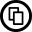
\includegraphics[scale=.5]{T0/cc-share.png}}]
Copiar, distribuir y comunicar públicamente la obra.
\item[\raisebox{-.5em}{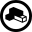
\includegraphics[scale=.5]{T0/cc-remix.png}}]
Hacer obras derivadas.
\end{itemize}
\item[Bajo las condiciones siguientes:]\ \par\vspace{-.6em}
\begin{itemize}
\item[\raisebox{-.5em}{
\includegraphics[scale=.5]{T0/cc-by-new.png}}]
\textbf{Reconocimiento.}
Debe reconocer los créditos de la obra de la manera especificada por el autor o el licenciador (pero no de una manera que sugiera que tiene su apoyo o apoyan el uso que hace de su obra).
\item[\raisebox{-.5em}{
\includegraphics[scale=.5]{T0/cc-nc-euro.png}}]
\textbf{No comercial.}
No puede utilizar esta obra para fines comerciales.
\item[\raisebox{-.5em}{
\includegraphics[scale=.5]{T0/cc-sa.png}}]
\textbf{Compartir bajo la misma licencia.}
Si altera o transforma esta obra, o genera una obra derivada, sólo puede distribuir la obra generada bajo una licencia idéntica a ésta.
\end{itemize}
\end{description}
\begin{itemize}
\item
Al reutilizar o distribuir la obra, tiene que dejar bien claro los términos de la licencia de esta obra.
\item
Alguna de estas condiciones puede no aplicarse si se obtiene el permiso del titular de los derechos de autor.
\item
Nada en esta licencia menoscaba o restringe los derechos morales del autor.
\end{itemize}
\end{minipage}

%\newpage
%
%\thispagestyle{plain}
%%\noindent{\large\textbf{Introducción}}
%
%\ \vspace{.2\textheight}
%
%\hfill\begin{minipage}{.5\textwidth}
%\em
%Yo no enseño a mis alumnos, solo les proporciono las condiciones en las que puedan aprender.
%
%\ \hfill
%Albert Einstein
%\end{minipage}
%
%%\ \vspace{.1\textheight}
%\ \vspace{4em}
%
%Este libro está concebido como una ``guía docente'' para la asignatura \emph{Cálculo para la computación} que se imparte en los tres grados que oferta la E.~T.~S.~I.~Informática de la Universidad de Málaga a partir del curso 2010/11.
%Su contenido es fruto del trabajo de varios años, previos a la redacción de los correspondientes planes de estudio, y en él han participado todos los profesores que durante este tiempo han impartido dicha asignatura.
%
%A lo largo de estos años, se ha ido rediseñando, curso a curso, la asignatura.
%Varios son los factores que han intervenido en este proceso.
%En primer lugar, se ha adecuado el contenido de cada tema a las necesidades reales de un futuro graduado en informática, intensificando o relajando los contenidos de cada apartado en función de ello.
%En segundo lugar, se ha buscado adaptar la curva de aprendizaje de los alumnos a su base real de conocimientos y al tiempo que los planes de estudio estiman necesarios para  preparar la asignatura.
%Posiblemente, este ha sido el factor más importante en el proceso de adaptación de los planes de estudio al Espacio Europeo de Educación Superior y el que más ha influido en el resultado final del programa que esta guía desarrolla.
%
%La estructura del libro se adapta a los objetivos establecidos para su creación.
%El contenido se divide en ``temas'', no en ``capítulos'', y cada tema se divide en ``lecciones'', no en secciones. Cada tema se inicia con una descripción en términos docentes: se detallan los objetivos, los prerrequisitos y se da un esquema de su contenido.
%
%%Cada tema concluye con dos relaciones de ejercicios.
%%La primera debe considerarse básica, contiene ejercicios de dificultad baja y media;
%%estos ejercicios deben ser resueltos por el alumno a medida que estudia el tema.
%%La segunda relación contiene ejercicios cuya dificultad se ajusta a los objetivos perseguidos y deben ser resueltos por el alumno para completar el estudio óptimo de la unidad temática.
%%Cada alumno debería elegir la cantidad final de ejercicios a resolver, en función de la facilidad o dificultad que encuentre al abordar el estudio de cada una de las partes de los temas.
%
%Esta asignatura, tiene asignados 6 créditos E.C.T.S.%
%\footnote{E.C.T.S. son la siglas de \emph{European Credit Transfer System}, es decir, Sistema Europeo de Transferencia de Créditos.}
%En los documentos que desarrollan los planes de estudio de los diferentes grados, esta asignación de créditos se traducen en una dedicación de 150 horas por parte del alumno.
%Es decir, se entiende que un alumno ``medio'' necesitará aproximadamente 150 horas de trabajo total para prepararse y superar la asignatura, incluyendo las que emplee en el aula, laboratorios o exámenes.
%No vamos a entrar aquí en las dificultades al valorar todas las fases del trabajo del alumno, de sus necesidades específicas o la calidad de las horas de estudio, pero en cualquier caso, en la elaboración de este documento se ha intentado ajustar los contenidos de la asignatura a este tiempo de dedicación.
%Sin embargo, es evidente que un alumno concreto deberá incrementar o podrá reducir este tiempo de trabajo en función de su formación previa y de la ``calidad'' de las horas de estudio, ya sea en casa o en clase.
%
%La distribución de los contenidos del curso abandona, en algunos momentos, lo que puede considerarse una estructura clásica de un curso de cálculo; además, también se han eliminado secciones que, aunque aparecen habitualmente en este tipo de cursos, consideramos que son más propias de estudiantes de matemáticas puras.
%Por ejemplo, la lección dedicada a las ecuaciones diferenciales se plantea como continuación al cálculo de primitivas, ya que ambos temas comparten técnicas, y la resolución de ecuaciones diferenciales se sustenta en el cálculo de primitivas.
%%Otro ejemplo destacable es que la integración se trata en el segundo tema desde el punto de vista numérico y posteriormente en el último tema para profundizar en su estudio.
%
%En el diseño de la asignatura se han seguido dos importantes premisas.
%Por un lado, se pretende que las destrezas a desarrollar por el alumno tengan dificultad ascendente, y para ello intentamos que, en la medida de lo posible, cada lección use, y por lo tanto refuerce, los contenidos de las lecciones anteriores.
%Por otra parte, se ha evitado incluir, de forma exhaustiva, los contenidos que un alumno que accede a la universidad debería conocer por su formación preuniversitaria;
%sin embargo, en cada tema se dedicará parte del tiempo a recordar estos contenidos, pero siempre vinculado al desarrollo de nuevos conceptos.
%
%%Finalmente, me gustaría destacar una restricción adoptada durante la elección de los contenidos.
%%A lo largo del curso, siempre trabajaremos con funciones expresadas en términos de funciones elementales y en consecuencia continuas y diferenciables.
%%Desde el punto de vista matemático, se puede entender que esta restricción es demasiado fuerte, pero entendemos que las condiciones actuales de la formación previa del alumno y el limitado peso que las asignaturas de matemáticas tienen en las nuevas titulaciones, obligan a optar por una formación intensiva.
%%De esta forma, entendemos que es preferible que el alumno conozca los diferentes modelos sobre funciones y ejemplos asequibles, dando una formación básica para futuros estudios más avanzados.
%
%
%%*** Revisar posteriormente: ***
%%Puede resultar extraño que el tema dedicado al estudio de los campos escalares no incluya un estudio formal de los conceptos de límite y de diferenciabilidad.
%%En dicho tema, nos centramos en el estudio de las propiedades de los campos continuos y diferenciales y en las aplicaciones de dichos conceptos.
%%Entendemos que es necesario que un estudiante de cálculo conozca en profundidad las funciones continuas y diferenciables antes de enfrentarse al análisis de casos ``excepcionales''.
%%
%%
%%\begin{itemize}
%%\item
%%No se estudian ni calculan límites de funciones de una variable.- L'Hôpital
%%
%%\item
%%No se estudían límites de campos. Solo trabajaremos con funciones continuas y diferenciables. Concretamente, funciones expresables mediante operaciones algebraicas entre funciones elementales.
%%
%%\item
%%El curso esta pensado para que el alumno estudie con la ayuda de software matemático.
%%Esta es una apuesta moderna que nos atrevemos a considerar necesaria.
%%El momento en el que nos encontramos es equiparable a cuando se decidió abandonar el uso de tablas para calcular logaritmos o funciones trigonométricas o se dejo de enseñar en las escuelas a calcular raíces cuadradas. 
%%Ahora nos encontramos en el momento en el que tenemos que decidir que cálculos matemáticos se dejan a los ordenadores y a los potentes, pero muy asequibles, programas de cálculo matemático.
%%
%%\begin{itemize}
%%\item
%%La resolución de ecuaciones y sistemas de ecuaciones responde a manipulaciones mecánicas o a heurísticas. Se deben conocer los fundamentos, pero adquirir la habilidad necesaria requiere mucho tiempo. 
%%
%%\item
%%Derivación. Aunque las reglas de derivación son imprescindibles, la derivación de funciones con expresiones más complejas y su posterior simplificación puede y debe hacerse con ordenador.
%%
%%\item
%%Cálculo de primitivas.
%%
%%\end{itemize}
%%\end{itemize}
%%
%%\newpage
%%
%%\ \thispagestyle{empty}
%%\setcounter{tocdepth}{3}
\setcounter{tocdepth}{1}

\tableofcontents

\newpage

\ \thispagestyle{empty}
